% Options for packages loaded elsewhere
\PassOptionsToPackage{unicode}{hyperref}
\PassOptionsToPackage{hyphens}{url}
\PassOptionsToPackage{dvipsnames,svgnames,x11names}{xcolor}
%
\documentclass[
  letterpaper,
  DIV=11,
  numbers=noendperiod]{scrartcl}

\usepackage{amsmath,amssymb}
\usepackage{iftex}
\ifPDFTeX
  \usepackage[T1]{fontenc}
  \usepackage[utf8]{inputenc}
  \usepackage{textcomp} % provide euro and other symbols
\else % if luatex or xetex
  \usepackage{unicode-math}
  \defaultfontfeatures{Scale=MatchLowercase}
  \defaultfontfeatures[\rmfamily]{Ligatures=TeX,Scale=1}
\fi
\usepackage{lmodern}
\ifPDFTeX\else  
    % xetex/luatex font selection
\fi
% Use upquote if available, for straight quotes in verbatim environments
\IfFileExists{upquote.sty}{\usepackage{upquote}}{}
\IfFileExists{microtype.sty}{% use microtype if available
  \usepackage[]{microtype}
  \UseMicrotypeSet[protrusion]{basicmath} % disable protrusion for tt fonts
}{}
\makeatletter
\@ifundefined{KOMAClassName}{% if non-KOMA class
  \IfFileExists{parskip.sty}{%
    \usepackage{parskip}
  }{% else
    \setlength{\parindent}{0pt}
    \setlength{\parskip}{6pt plus 2pt minus 1pt}}
}{% if KOMA class
  \KOMAoptions{parskip=half}}
\makeatother
\usepackage{xcolor}
\setlength{\emergencystretch}{3em} % prevent overfull lines
\setcounter{secnumdepth}{4}
% Make \paragraph and \subparagraph free-standing
\makeatletter
\ifx\paragraph\undefined\else
  \let\oldparagraph\paragraph
  \renewcommand{\paragraph}{
    \@ifstar
      \xxxParagraphStar
      \xxxParagraphNoStar
  }
  \newcommand{\xxxParagraphStar}[1]{\oldparagraph*{#1}\mbox{}}
  \newcommand{\xxxParagraphNoStar}[1]{\oldparagraph{#1}\mbox{}}
\fi
\ifx\subparagraph\undefined\else
  \let\oldsubparagraph\subparagraph
  \renewcommand{\subparagraph}{
    \@ifstar
      \xxxSubParagraphStar
      \xxxSubParagraphNoStar
  }
  \newcommand{\xxxSubParagraphStar}[1]{\oldsubparagraph*{#1}\mbox{}}
  \newcommand{\xxxSubParagraphNoStar}[1]{\oldsubparagraph{#1}\mbox{}}
\fi
\makeatother

\usepackage{color}
\usepackage{fancyvrb}
\newcommand{\VerbBar}{|}
\newcommand{\VERB}{\Verb[commandchars=\\\{\}]}
\DefineVerbatimEnvironment{Highlighting}{Verbatim}{commandchars=\\\{\}}
% Add ',fontsize=\small' for more characters per line
\newenvironment{Shaded}{}{}
\newcommand{\AlertTok}[1]{\textcolor[rgb]{0.58,0.85,0.30}{\textbf{\colorbox[rgb]{0.30,0.12,0.14}{#1}}}}
\newcommand{\AnnotationTok}[1]{\textcolor[rgb]{0.31,0.63,0.31}{#1}}
\newcommand{\AttributeTok}[1]{\textcolor[rgb]{0.65,0.15,0.64}{#1}}
\newcommand{\BaseNTok}[1]{\textcolor[rgb]{0.60,0.41,0.00}{#1}}
\newcommand{\BuiltInTok}[1]{\textcolor[rgb]{0.65,0.15,0.64}{#1}}
\newcommand{\CharTok}[1]{\textcolor[rgb]{0.31,0.63,0.31}{#1}}
\newcommand{\CommentTok}[1]{\textcolor[rgb]{0.63,0.63,0.65}{\textit{#1}}}
\newcommand{\CommentVarTok}[1]{\textcolor[rgb]{0.89,0.34,0.29}{\textit{#1}}}
\newcommand{\ConstantTok}[1]{\textcolor[rgb]{0.60,0.41,0.00}{#1}}
\newcommand{\ControlFlowTok}[1]{\textcolor[rgb]{0.65,0.15,0.64}{#1}}
\newcommand{\DataTypeTok}[1]{\textcolor[rgb]{0.65,0.15,0.64}{#1}}
\newcommand{\DecValTok}[1]{\textcolor[rgb]{0.60,0.41,0.00}{#1}}
\newcommand{\DocumentationTok}[1]{\textcolor[rgb]{0.89,0.34,0.29}{#1}}
\newcommand{\ErrorTok}[1]{\textcolor[rgb]{0.96,0.28,0.28}{\underline{#1}}}
\newcommand{\ExtensionTok}[1]{\textcolor[rgb]{0.25,0.47,0.95}{\textbf{#1}}}
\newcommand{\FloatTok}[1]{\textcolor[rgb]{0.60,0.41,0.00}{#1}}
\newcommand{\FunctionTok}[1]{\textcolor[rgb]{0.25,0.47,0.95}{#1}}
\newcommand{\ImportTok}[1]{\textcolor[rgb]{0.31,0.63,0.31}{#1}}
\newcommand{\InformationTok}[1]{\textcolor[rgb]{0.77,0.36,0.00}{#1}}
\newcommand{\KeywordTok}[1]{\textcolor[rgb]{0.65,0.15,0.64}{#1}}
\newcommand{\NormalTok}[1]{\textcolor[rgb]{0.22,0.23,0.26}{#1}}
\newcommand{\OperatorTok}[1]{\textcolor[rgb]{0.65,0.15,0.64}{#1}}
\newcommand{\OtherTok}[1]{\textcolor[rgb]{0.15,0.68,0.38}{#1}}
\newcommand{\PreprocessorTok}[1]{\textcolor[rgb]{0.65,0.15,0.64}{#1}}
\newcommand{\RegionMarkerTok}[1]{\textcolor[rgb]{0.16,0.50,0.73}{\colorbox[rgb]{0.08,0.19,0.26}{#1}}}
\newcommand{\SpecialCharTok}[1]{\textcolor[rgb]{0.00,0.52,0.74}{#1}}
\newcommand{\SpecialStringTok}[1]{\textcolor[rgb]{0.85,0.27,0.33}{#1}}
\newcommand{\StringTok}[1]{\textcolor[rgb]{0.31,0.63,0.31}{#1}}
\newcommand{\VariableTok}[1]{\textcolor[rgb]{0.89,0.34,0.29}{#1}}
\newcommand{\VerbatimStringTok}[1]{\textcolor[rgb]{0.85,0.27,0.33}{#1}}
\newcommand{\WarningTok}[1]{\textcolor[rgb]{0.85,0.27,0.33}{#1}}

\providecommand{\tightlist}{%
  \setlength{\itemsep}{0pt}\setlength{\parskip}{0pt}}\usepackage{longtable,booktabs,array}
\usepackage{calc} % for calculating minipage widths
% Correct order of tables after \paragraph or \subparagraph
\usepackage{etoolbox}
\makeatletter
\patchcmd\longtable{\par}{\if@noskipsec\mbox{}\fi\par}{}{}
\makeatother
% Allow footnotes in longtable head/foot
\IfFileExists{footnotehyper.sty}{\usepackage{footnotehyper}}{\usepackage{footnote}}
\makesavenoteenv{longtable}
\usepackage{graphicx}
\makeatletter
\def\maxwidth{\ifdim\Gin@nat@width>\linewidth\linewidth\else\Gin@nat@width\fi}
\def\maxheight{\ifdim\Gin@nat@height>\textheight\textheight\else\Gin@nat@height\fi}
\makeatother
% Scale images if necessary, so that they will not overflow the page
% margins by default, and it is still possible to overwrite the defaults
% using explicit options in \includegraphics[width, height, ...]{}
\setkeys{Gin}{width=\maxwidth,height=\maxheight,keepaspectratio}
% Set default figure placement to htbp
\makeatletter
\def\fps@figure{htbp}
\makeatother

\usepackage{setspace}
\usepackage[most]{tcolorbox}

\newtcolorbox{note}{
	colback=gray!10,
	colframe=gray!80!black,
	boxrule=0.5pt,
	arc=2mm,
	left=6pt,
	right=6pt,
	top=6pt,
	bottom=6pt,
	enhanced,
	before upper={\setstretch{1.2}},
}

\newtcolorbox{example}{
	colback=blue!10,
	colframe=blue!80!black,
	boxrule=0.5pt,
	arc=2mm,
	left=6pt,
	right=6pt,
	top=6pt,
	bottom=6pt,
	enhanced,
	before upper={\setstretch{1.2}},
}

% \usepackage[most]{tcolorbox}
% \newtcolorbox{shadednote}{
%   colback=gray!10,
%   colframe=gray!80!black,
%   boxrule=0.5pt,
%   arc=2mm,
%   left=6pt,
%   right=6pt,
%   top=6pt,
%   bottom=6pt,
%   enhanced,
%   before upper=\relax, % Do nothing, let it inherit
% }
% \newtcolorbox{shadednote}{
%   colback=gray!10,
%   colframe=gray!80!black,
%   boxrule=0.5pt,
%   arc=2mm,
%   left=6pt,
%   right=6pt,
%   top=6pt,
%   bottom=6pt,
% }
\usepackage{booktabs}
\usepackage{longtable}
\usepackage{array}
\usepackage{multirow}
\usepackage{wrapfig}
\usepackage{float}
\usepackage{colortbl}
\usepackage{pdflscape}
\usepackage{tabu}
\usepackage{threeparttable}
\usepackage{threeparttablex}
\usepackage[normalem]{ulem}
\usepackage{makecell}
\usepackage{xcolor}
\KOMAoption{captions}{tableheading}
\makeatletter
\@ifpackageloaded{caption}{}{\usepackage{caption}}
\AtBeginDocument{%
\ifdefined\contentsname
  \renewcommand*\contentsname{Table of contents}
\else
  \newcommand\contentsname{Table of contents}
\fi
\ifdefined\listfigurename
  \renewcommand*\listfigurename{List of Figures}
\else
  \newcommand\listfigurename{List of Figures}
\fi
\ifdefined\listtablename
  \renewcommand*\listtablename{List of Tables}
\else
  \newcommand\listtablename{List of Tables}
\fi
\ifdefined\figurename
  \renewcommand*\figurename{Figure}
\else
  \newcommand\figurename{Figure}
\fi
\ifdefined\tablename
  \renewcommand*\tablename{Table}
\else
  \newcommand\tablename{Table}
\fi
}
\@ifpackageloaded{float}{}{\usepackage{float}}
\floatstyle{ruled}
\@ifundefined{c@chapter}{\newfloat{codelisting}{h}{lop}}{\newfloat{codelisting}{h}{lop}[chapter]}
\floatname{codelisting}{Listing}
\newcommand*\listoflistings{\listof{codelisting}{List of Listings}}
\makeatother
\makeatletter
\makeatother
\makeatletter
\@ifpackageloaded{caption}{}{\usepackage{caption}}
\@ifpackageloaded{subcaption}{}{\usepackage{subcaption}}
\makeatother
\makeatletter
\@ifpackageloaded{tcolorbox}{}{\usepackage[skins,breakable]{tcolorbox}}
\makeatother
\makeatletter
\@ifundefined{shadecolor}{\definecolor{shadecolor}{named}{white}}{}
\makeatother
\makeatletter
\@ifundefined{codebgcolor}{\definecolor{codebgcolor}{HTML}{f8f8f8}}{}
\makeatother
\makeatletter
\ifdefined\Shaded\renewenvironment{Shaded}{\begin{tcolorbox}[borderline west={3pt}{0pt}{shadecolor}, boxrule=0pt, enhanced, sharp corners, colback={codebgcolor}, frame hidden, breakable]}{\end{tcolorbox}}\fi
\makeatother

\ifLuaTeX
  \usepackage{selnolig}  % disable illegal ligatures
\fi
\usepackage{bookmark}

\IfFileExists{xurl.sty}{\usepackage{xurl}}{} % add URL line breaks if available
\urlstyle{same} % disable monospaced font for URLs
\hypersetup{
  pdftitle={Understanding Jacobian Adjustments for Constrained Parameters in Stan},
  pdfauthor={Yingqi Jing},
  colorlinks=true,
  linkcolor={blue},
  filecolor={Maroon},
  citecolor={Blue},
  urlcolor={Blue},
  pdfcreator={LaTeX via pandoc}}


\title{Understanding Jacobian Adjustments for Constrained Parameters in
Stan}
\author{Yingqi Jing}
\date{July 21, 2025}

\begin{document}
\maketitle

\renewcommand*\contentsname{Contents}
{
\hypersetup{linkcolor=}
\setcounter{tocdepth}{4}
\tableofcontents
}
\listoffigures
\listoftables

\clearpage

\section{Normal distribution}\label{normal-distribution}

\begin{figure}[H]

{\centering 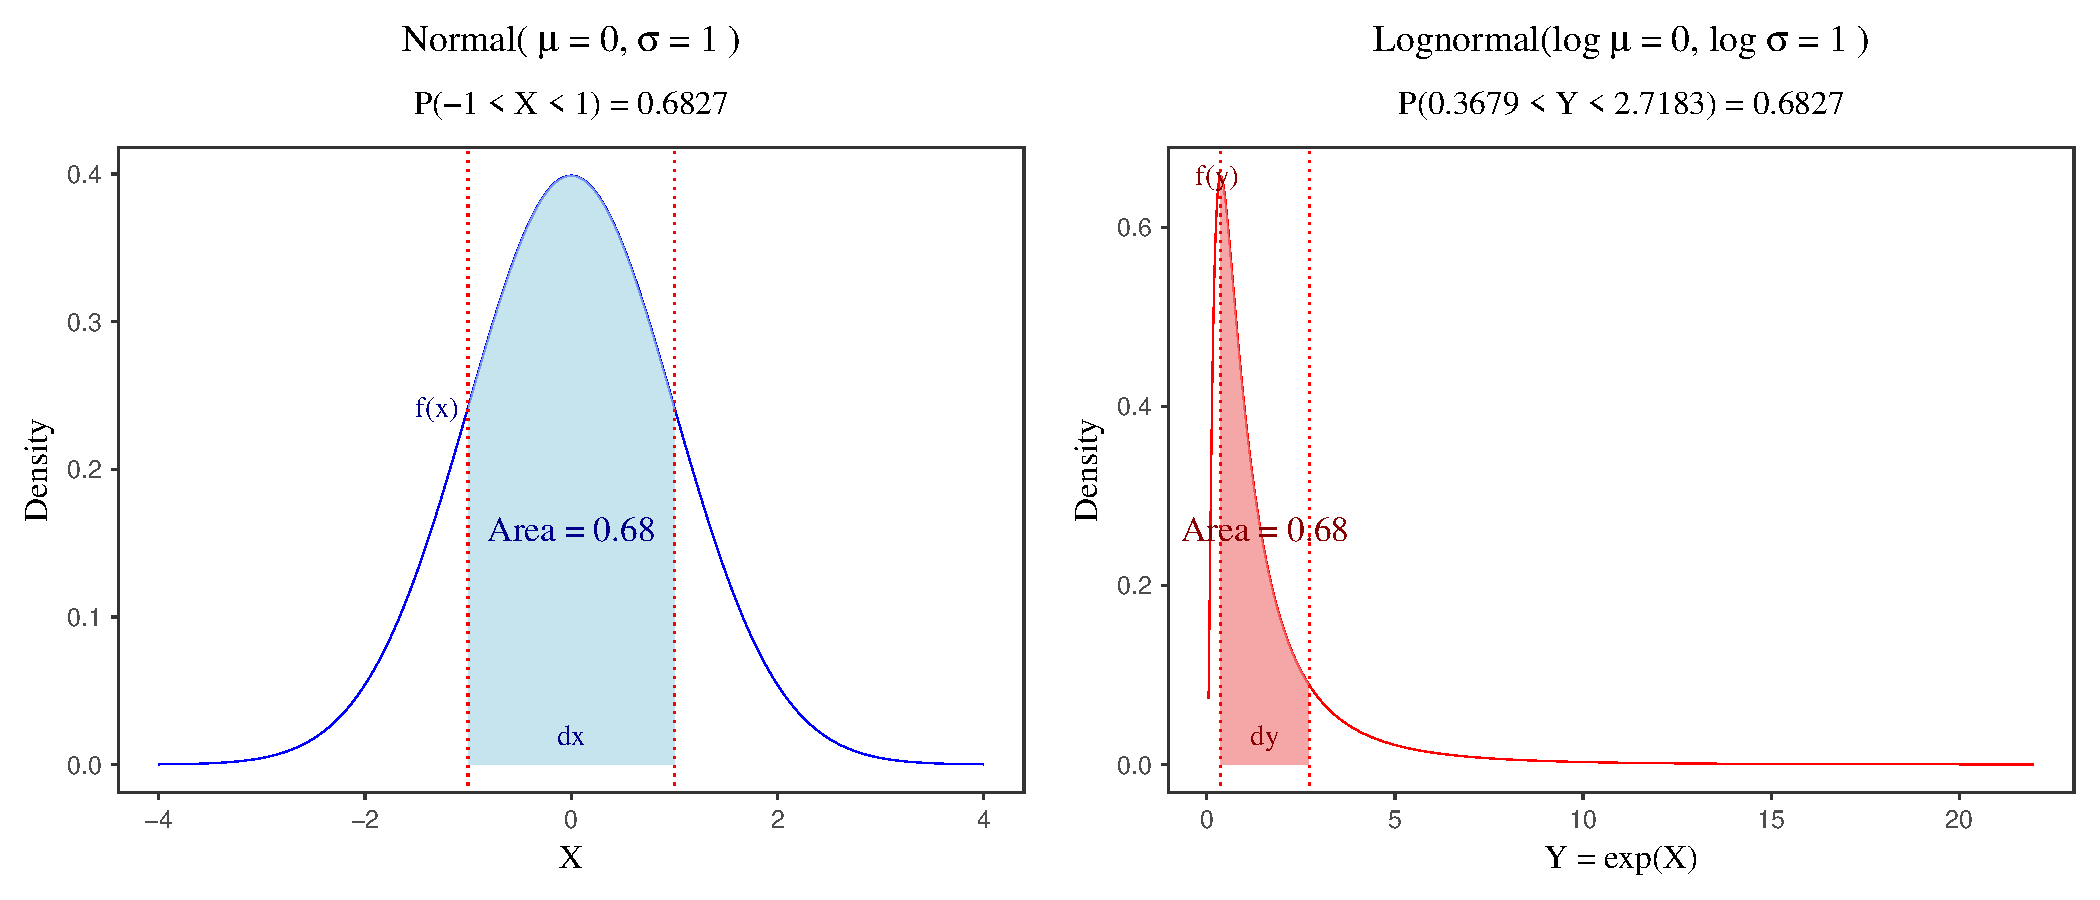
\includegraphics{figures/unnamed-chunk-1-1.pdf}

}

\caption{Probability masses of normal and lognormal distributions within
the corresponding intervals}

\end{figure}%

The Jacobian adjustment is a key concept in statistical modeling that
arises when transforming probability distributions from one space to
another. The intuition is that when you change a random variable, you're
not just changing the values - you're also changing how ``stretched'' or
``compressed'' the probability density becomes at different points. To
account for the distortion caused by the transform, the density must be
multiplied by a Jacobian adjustment. This ensures that probability
masses of corresponding intervals stay unchanged before and after the
transform. This is illustrated by the figure above, which compares the
probability density functions of a standard normal distribution and its
transformed lognormal distribution. Although the shapes of the two
distributions differ, the transformation must preserve the probability
mass over corresponding intervals.

In Bayesian inference, Jacobian adjustments are especially important
when transforming parameters from a constrained space (e.g., the
positive real line) to an unconstrained space (e.g., the entire real
line), which is commonly done to improve sampling efficiency and
numerical stability. In Stan, such transformations are typically handled
automatically. When you declare a constrained parameter (e.g.,
\textless lower=0\textgreater), Stan internally transforms it to an
unconstrained space and applies the appropriate Jacobian adjustment to
maintain the correct posterior density.

However, if you manually transform variables inside the transformed
parameters block and assign priors to the transformed variables, you
need to explicitly include the Jacobian adjustment to preserve the
correct log posterior density (lp\_\_). Failing to do so can lead to
biased inference. To illustrate how this works, I'll use a simple
example of normal distribution, focusing on how Stan handles
transformations of the standard deviation parameter \(\sigma\) (i.e.,
\textless lower=0\textgreater) and how we can include a manual Jacobian
adjustment.

\subsection{Simulate data}\label{simulate-data}

I will first simulate some data from a normal distribution with mean 0
and standard deviation 20. A large standard deviation is chosen to make
the effect of Jacobian adjustment more pronounced.

\begin{Shaded}
\begin{Highlighting}[]
\NormalTok{data\_norm }\OtherTok{\textless{}{-}} \FunctionTok{list}\NormalTok{(}\AttributeTok{N =} \DecValTok{100}\NormalTok{, }\AttributeTok{y =} \FunctionTok{rnorm}\NormalTok{(}\DecValTok{100}\NormalTok{, }\DecValTok{0}\NormalTok{, }\DecValTok{20}\NormalTok{))}
\end{Highlighting}
\end{Shaded}

\subsection{Posterior parameter
estimates}\label{posterior-parameter-estimates}

I will include four models to compare posterior parameter estimates and
the log posterior density (lp\_\_). The models are:

Model 1: A normal distribution with a proper constraint on \(\sigma\)
Model 2: A normal distribution without a constraint on \(\sigma\) Model
3: A normal distribution with an exponential transformation of
unconstrained \(\sigma_z\) and a Jacobian adjustment Model 4: A normal
distribution with transformation of \(\sigma\) in the transformed
parameters block (No Jacobian needed!)

\subsubsection{\texorpdfstring{Model 1: constrained
\(\sigma\)}{Model 1: constrained \textbackslash sigma}}\label{model-1-constrained-sigma}

The first model is a simple normal distribution with a proper constraint
on \(\sigma\) (\textless lower=0\textgreater). According to
\href{https://mc-stan.org/docs/reference-manual/transforms.html}{Stan
reference manual}, to avoid having to deal with constraints while
simulating the Hamiltonian dynamics during sampling, every
(multivariate) parameter in a Stan model is transformed to an
unconstrained variable behind the scenes by the model compiler, and Stan
handles the Jacobian adjustment automatically.

\begin{Shaded}
\begin{Highlighting}[]
\KeywordTok{data}\NormalTok{ \{}
  \DataTypeTok{int}\NormalTok{\textless{}}\KeywordTok{lower}\NormalTok{=}\DecValTok{0}\NormalTok{\textgreater{} N; }\CommentTok{// number of observations}
  \DataTypeTok{vector}\NormalTok{[N] y; }\CommentTok{// observed data}
\NormalTok{\}}

\KeywordTok{parameters}\NormalTok{ \{}
  \DataTypeTok{real}\NormalTok{ mu; }\CommentTok{// mean parameter}
  \DataTypeTok{real}\NormalTok{\textless{}}\KeywordTok{lower}\NormalTok{=}\DecValTok{0}\NormalTok{\textgreater{} sigma; }\CommentTok{// standard deviation parameter}
\NormalTok{\}}

\KeywordTok{model}\NormalTok{ \{}
  \CommentTok{// Priors}
  \KeywordTok{target +=}\NormalTok{ normal\_lpdf(mu | }\DecValTok{0}\NormalTok{, }\DecValTok{10}\NormalTok{); }\CommentTok{// prior for mean}
  \KeywordTok{target +=}\NormalTok{ normal\_lpdf(sigma | }\DecValTok{0}\NormalTok{, }\DecValTok{5}\NormalTok{); }\CommentTok{// prior for standard deviation}
  
  \CommentTok{// Likelihood}
  \KeywordTok{target +=}\NormalTok{ normal\_lpdf(y | mu, sigma); }\CommentTok{// data follows normal distribution}
\NormalTok{\}}
\end{Highlighting}
\end{Shaded}

\begin{Shaded}
\begin{Highlighting}[]
\NormalTok{md\_norm }\OtherTok{\textless{}{-}} \FunctionTok{stan\_model}\NormalTok{(}\AttributeTok{file =} \StringTok{"./Models/normal.stan"}\NormalTok{)}
\NormalTok{fit\_norm }\OtherTok{\textless{}{-}} \FunctionTok{sampling}\NormalTok{(md\_norm, data\_norm,}
  \AttributeTok{iter =} \DecValTok{2000}\NormalTok{, }\AttributeTok{chains =} \DecValTok{1}
\NormalTok{)}
\FunctionTok{print}\NormalTok{(fit\_norm, }\AttributeTok{pars =} \FunctionTok{c}\NormalTok{(}\StringTok{"mu"}\NormalTok{, }\StringTok{"sigma"}\NormalTok{, }\StringTok{"lp\_\_"}\NormalTok{))}
\end{Highlighting}
\end{Shaded}

\subsubsection{\texorpdfstring{Model 2: unconstrained
\(\sigma\)}{Model 2: unconstrained \textbackslash sigma}}\label{model-2-unconstrained-sigma}

Now we turn to another model by removing the constraint on \(\sigma\).
In this case, the parameter \(\sigma\) is not a constrained variable,
and there is no Jacobian adjustment handled by Stan. This means that the
log posterior density (lp\_\_) is biased.

\begin{Shaded}
\begin{Highlighting}[]
\KeywordTok{data}\NormalTok{ \{}
  \DataTypeTok{int}\NormalTok{\textless{}}\KeywordTok{lower}\NormalTok{=}\DecValTok{0}\NormalTok{\textgreater{} N; }\CommentTok{// number of observations}
  \DataTypeTok{vector}\NormalTok{[N] y; }\CommentTok{// observed data}
\NormalTok{\}}

\KeywordTok{parameters}\NormalTok{ \{}
  \DataTypeTok{real}\NormalTok{ mu; }\CommentTok{// mean parameter}
  \DataTypeTok{real}\NormalTok{ sigma; }\CommentTok{// standard deviation parameter}
\NormalTok{\}}
\KeywordTok{model}\NormalTok{ \{}
  \CommentTok{// Priors}
  \KeywordTok{target +=}\NormalTok{ normal\_lpdf(mu | }\DecValTok{0}\NormalTok{, }\DecValTok{10}\NormalTok{); }\CommentTok{// prior for mean}
  \KeywordTok{target +=}\NormalTok{ normal\_lpdf(sigma | }\DecValTok{0}\NormalTok{, }\DecValTok{5}\NormalTok{); }\CommentTok{// prior for standard deviation}
  
  \CommentTok{// Likelihood}
  \KeywordTok{target +=}\NormalTok{ normal\_lpdf(y | mu, sigma); }\CommentTok{// data follows normal distribution}
\NormalTok{\}}
\end{Highlighting}
\end{Shaded}

\begin{Shaded}
\begin{Highlighting}[]
\NormalTok{md\_norm\_no\_constraint }\OtherTok{\textless{}{-}} \FunctionTok{stan\_model}\NormalTok{(}\AttributeTok{file =} \StringTok{"./Models/normal\_no\_constraint\_sigma.stan"}\NormalTok{)}
\NormalTok{fit\_norm\_no\_constraint }\OtherTok{\textless{}{-}} \FunctionTok{sampling}\NormalTok{(md\_norm\_no\_constraint, data\_norm,}
  \AttributeTok{iter =} \DecValTok{2000}\NormalTok{, }\AttributeTok{chains =} \DecValTok{1}
\NormalTok{)}
\FunctionTok{print}\NormalTok{(fit\_norm\_no\_constraint, }\AttributeTok{pars =} \FunctionTok{c}\NormalTok{(}\StringTok{"mu"}\NormalTok{, }\StringTok{"sigma"}\NormalTok{, }\StringTok{"lp\_\_"}\NormalTok{))}
\end{Highlighting}
\end{Shaded}

\subsubsection{\texorpdfstring{Model 3: exponential transformation of
unconstrained \(\sigma_z\) and Jacobian
adjustment}{Model 3: exponential transformation of unconstrained \textbackslash sigma\_z and Jacobian adjustment}}\label{model-3-exponential-transformation-of-unconstrained-sigma_z-and-jacobian-adjustment}

As a comparison, we can also reformulate the model by defining the
parameter \(\sigma_z\) as an unconstrained variable, and we then
transform it via an exponential function (positive real line). The
transformed variable \(\sigma\) will be assigned with a prior and used
in the model. This is exactly what has happened internally by Stan when
you define a parameter with a proper constraint (e.g.,
\textless lower=0\textgreater{} for \(\sigma\)). Stan handles the
transformation from an unconstrained internal representation to this
constrained user-facing value. Since \(\sigma\) is transformed from
\(\sigma_z\), we need to include a Jacobian adjustment to preserve the
correct log posterior density (lp\_\_).

\begin{note}
Let me explain how the Jacobian adjustment works step by step.

Let:
$$
y = \sigma_e, \quad x = \sigma, \quad y = \exp(x)
$$

We are transforming from an unconstrained variable $ x \in \mathbb{R} $ to a positive variable $ y \in (0, \infty) $.

Next, we can compute the derivative:
$$
\frac{dy}{dx} = \frac{d}{dx} \exp(x) = \exp(x) = y
$$

We apply the change-of-variables formula for densities:
$$
\left|f_Y(y) \cdot dy\right| = \left|f_X(x) \cdot dx\right| 
\quad \Rightarrow \quad 
f_Y(y) \cdot \left| \frac{dy}{dx} \right| = f_X(x)
$$

Substituting $ \frac{dy}{dx} = y $, we get:
$$
f_Y(y) \cdot y = f_X(x)
$$

Taking logs to get log-densities:
$$
\log f_X(x) = \log f_Y(y) + \log y
$$

This extra term $ \log y $ is the \textbf{Jacobian adjustment}.

In Stan notation, we get:

$$
\text{target} ~ \text{+=} ~ \text{normal\_lpdf}(\mu, \exp(\sigma_e)) + \log(\sigma_e)
$$
\end{note}

\begin{Shaded}
\begin{Highlighting}[]
\KeywordTok{data}\NormalTok{ \{}
  \DataTypeTok{int}\NormalTok{\textless{}}\KeywordTok{lower}\NormalTok{=}\DecValTok{0}\NormalTok{\textgreater{} N; }\CommentTok{// number of observations}
  \DataTypeTok{vector}\NormalTok{[N] y; }\CommentTok{// observed data}
\NormalTok{\}}
\KeywordTok{parameters}\NormalTok{ \{}
  \DataTypeTok{real}\NormalTok{ mu; }\CommentTok{// mean parameter}
  \DataTypeTok{real}\NormalTok{ sigma\_z; }\CommentTok{// unconstrained standard deviation parameter}
\NormalTok{\}}
\KeywordTok{transformed parameters}\NormalTok{ \{}
  \DataTypeTok{real}\NormalTok{ sigma = exp(sigma\_z);}
\NormalTok{\}}
\KeywordTok{model}\NormalTok{ \{}
  \CommentTok{// Method 1: prior on sigma, with transformed block and Jacobian adjustment}
  \KeywordTok{target +=}\NormalTok{ normal\_lpdf(sigma | }\DecValTok{0}\NormalTok{, }\DecValTok{5}\NormalTok{); }\CommentTok{// prior for the transformed standard deviation}

  \CommentTok{// Method 2: local variable sigma, no transformed block, but with Jacobian adjustment}
  \CommentTok{// real sigma = exp(sigma\_z);}
  \CommentTok{// target += normal\_lpdf(sigma | 0, 5); // prior for the transformed standard deviation}

  \KeywordTok{target +=}\NormalTok{ normal\_lpdf(mu | }\DecValTok{0}\NormalTok{, }\DecValTok{10}\NormalTok{); }\CommentTok{// prior for mean}
  
  \CommentTok{// Likelihood}
  \KeywordTok{target +=}\NormalTok{ normal\_lpdf(y | mu, sigma) + log(sigma); }\CommentTok{// add Jacobian adjustment}
  \CommentTok{// target += normal\_lpdf(y | mu, sigma) + sigma\_z; // alternatively}
\NormalTok{\}}

\end{Highlighting}
\end{Shaded}

\begin{Shaded}
\begin{Highlighting}[]
\NormalTok{md\_norm\_exp\_jacobian }\OtherTok{\textless{}{-}} \FunctionTok{stan\_model}\NormalTok{(}\AttributeTok{file =} \StringTok{"./Models/normal\_exp\_sigma\_jacobian.stan"}\NormalTok{)}
\NormalTok{fit\_norm\_exp\_jacobian }\OtherTok{\textless{}{-}} \FunctionTok{sampling}\NormalTok{(md\_norm\_exp\_jacobian, data\_norm,}
  \AttributeTok{iter =} \DecValTok{2000}\NormalTok{, }\AttributeTok{chains =} \DecValTok{1}
\NormalTok{)}
\FunctionTok{print}\NormalTok{(fit\_norm\_exp\_jacobian, }\AttributeTok{pars =} \FunctionTok{c}\NormalTok{(}\StringTok{"mu"}\NormalTok{, }\StringTok{"lp\_\_"}\NormalTok{))}
\FunctionTok{print}\NormalTok{(fit\_norm\_exp\_jacobian, }\AttributeTok{pars =} \FunctionTok{c}\NormalTok{(}\StringTok{"mu"}\NormalTok{, }\StringTok{"sigma"}\NormalTok{, }\StringTok{"lp\_\_"}\NormalTok{))}
\end{Highlighting}
\end{Shaded}

\subsubsection{\texorpdfstring{Model 4: transformation of \(\sigma\) in
the transformed parameters block (No Jacobian
needed!)}{Model 4: transformation of \textbackslash sigma in the transformed parameters block (No Jacobian needed!)}}\label{model-4-transformation-of-sigma-in-the-transformed-parameters-block-no-jacobian-needed}

It is also worth mentioning that if you transform the parameter
\(\sigma\) in the transformed parameters block without assigning a prior
to the transformed parameter, you do not need to include a Jacobian
adjustment. This is because the transformation is applied to the
parameter after sampling. This is conceptually similar to generating
quantities from posterior draws.

As a general rule, if you place priors on the declared parameters or
directly use the parameters inside parameters block (in most cases),
rather than on transformed parameters, no Jacobian adjustment is
needed---this is a simple variable transformation. By contrast, if you
transform a parameter and place a prior on the transformed variable, you
need to include a Jacobian adjustment.

\begin{Shaded}
\begin{Highlighting}[]
\KeywordTok{data}\NormalTok{ \{}
  \DataTypeTok{int}\NormalTok{\textless{}}\KeywordTok{lower}\NormalTok{=}\DecValTok{0}\NormalTok{\textgreater{} N;}
  \DataTypeTok{vector}\NormalTok{[N] y;}
\NormalTok{\}}
\KeywordTok{parameters}\NormalTok{ \{}
  \DataTypeTok{real}\NormalTok{ mu;}
  \DataTypeTok{real}\NormalTok{\textless{}}\KeywordTok{lower}\NormalTok{=}\DecValTok{0}\NormalTok{\textgreater{} sigma;}
\NormalTok{\} }
\KeywordTok{transformed parameters}\NormalTok{ \{}
  \CommentTok{// Method 1: simple transformation without a prior for the transformed parameter}
  \DataTypeTok{real}\NormalTok{ log\_sigma = log(sigma); }
\NormalTok{\}}
\KeywordTok{model}\NormalTok{ \{}
  \CommentTok{// Priors}
  \KeywordTok{target +=}\NormalTok{ normal\_lpdf(mu | }\DecValTok{0}\NormalTok{, }\DecValTok{10}\NormalTok{);}
  \KeywordTok{target +=}\NormalTok{ normal\_lpdf(sigma | }\DecValTok{0}\NormalTok{, }\DecValTok{5}\NormalTok{); }\CommentTok{// prior on sigma}

  \CommentTok{// Likelihood}
  \KeywordTok{target +=}\NormalTok{ normal\_lpdf(y | mu, sigma);}
\NormalTok{\}}
\end{Highlighting}
\end{Shaded}

\begin{Shaded}
\begin{Highlighting}[]
\NormalTok{md\_norm\_transform\_parameters }\OtherTok{\textless{}{-}} \FunctionTok{stan\_model}\NormalTok{(}\AttributeTok{file =} \StringTok{"./Models/normal\_transform\_parameters.stan"}\NormalTok{)}
\NormalTok{fit\_norm\_transform\_parameters }\OtherTok{\textless{}{-}} \FunctionTok{sampling}\NormalTok{(md\_norm\_transform\_parameters, data\_norm,}
  \AttributeTok{iter =} \DecValTok{2000}\NormalTok{, }\AttributeTok{chains =} \DecValTok{1}
\NormalTok{)}
\FunctionTok{print}\NormalTok{(fit\_norm\_transform\_parameters, }\AttributeTok{pars =} \FunctionTok{c}\NormalTok{(}\StringTok{"mu"}\NormalTok{, }\StringTok{"sigma"}\NormalTok{, }\StringTok{"lp\_\_"}\NormalTok{))}
\end{Highlighting}
\end{Shaded}

\subsubsection{\texorpdfstring{Model 5: log transformation of \(\sigma\)
in the model block as a local variable (prior density changed, not
related to Jacobian
adjustment)}{Model 5: log transformation of \textbackslash sigma in the model block as a local variable (prior density changed, not related to Jacobian adjustment)}}\label{model-5-log-transformation-of-sigma-in-the-model-block-as-a-local-variable-prior-density-changed-not-related-to-jacobian-adjustment}

You may think of it in a different way by transforming the parameter
\(\sigma\) via logrithm transformation. This is not what happened under
the hood in stan, since Jacobian adjustment is performed on the absolute
derivative of the inverse transform. See the
\href{https://mc-stan.org/docs/reference-manual/transforms.html}{stan
reference manual} for more details.

\begin{note}
\textbf{Univariate changes of variables}
Suppose $X$ is one dimensional and $f : \mathrm{supp}(X) \to \mathbb{R}$ is a one-to-one, monotonic function with a differentiable inverse $f^{-1}$. Then the density of $Y$ is given by

$$
p_Y(y) = p_X(f^{-1}(y)) \left| \frac{d}{dy} f^{-1}(y) \right|
$$

The absolute derivative of the inverse transform measures how the scale of the transformed variable changes with respect to the underlying variable.
\end{note}

If you change in this way, you will change the prior on \(\sigma\). You
will not get the same log posterior density (lp\_\_) as Model 1, since
the prior on \(\sigma\) is different.

In model 1: \(\sigma \sim \mathcal{N}(0, 5)\)

In model 5: \(\log(\sigma) \sim \mathcal{N}(0, 5)\) or
\(\sigma \sim \mathcal{LogN}(0, 5)\)

My own opinion is that it is not recommended to transform the parameter
locally inside the model block, since (1) it is not that transparent
unless you really know what you are doing and (2) it will not be saved
in the output.

\begin{Shaded}
\begin{Highlighting}[]
\KeywordTok{data}\NormalTok{ \{}
  \DataTypeTok{int}\NormalTok{\textless{}}\KeywordTok{lower}\NormalTok{=}\DecValTok{0}\NormalTok{\textgreater{} N;}
  \DataTypeTok{vector}\NormalTok{[N] y;}
\NormalTok{\}}
\KeywordTok{parameters}\NormalTok{ \{}
  \DataTypeTok{real}\NormalTok{ mu;}
  \DataTypeTok{real}\NormalTok{\textless{}}\KeywordTok{lower}\NormalTok{=}\DecValTok{0}\NormalTok{\textgreater{} sigma;}
\NormalTok{\}}
\KeywordTok{model}\NormalTok{ \{}
  \CommentTok{// Method 1: prior on log(sigma) {-}{-}\textgreater{} lead to a different prior on sigma}
  \KeywordTok{target +=}\NormalTok{ normal\_lpdf(log(sigma) | }\DecValTok{0}\NormalTok{, }\DecValTok{5}\NormalTok{);}
  \KeywordTok{target +=}\NormalTok{ lognormal\_lpdf(sigma | }\DecValTok{0}\NormalTok{, }\DecValTok{5}\NormalTok{); }\CommentTok{// equivalently}

  \CommentTok{// Method 2: prior on local variable sigma\_log with Jacobian adjustment}
  \CommentTok{// real sigma\_log = log(sigma);}
  \CommentTok{// target += normal\_lpdf(sigma\_log | 0, 5);}

  \CommentTok{// Priors}
  \KeywordTok{target +=}\NormalTok{ normal\_lpdf(mu | }\DecValTok{0}\NormalTok{, }\DecValTok{10}\NormalTok{);}

  \CommentTok{// Likelihood}
  \KeywordTok{target +=}\NormalTok{ normal\_lpdf(y | mu, sigma);}
\NormalTok{\}}
\end{Highlighting}
\end{Shaded}

\begin{Shaded}
\begin{Highlighting}[]
\NormalTok{md\_norm\_transform\_local }\OtherTok{\textless{}{-}} \FunctionTok{stan\_model}\NormalTok{(}\AttributeTok{file =} \StringTok{"./Models/normal\_transform\_local.stan"}\NormalTok{)}
\NormalTok{fit\_norm\_transform\_local }\OtherTok{\textless{}{-}} \FunctionTok{sampling}\NormalTok{(md\_norm\_transform\_local, data\_norm,}
  \AttributeTok{iter =} \DecValTok{2000}\NormalTok{, }\AttributeTok{chains =} \DecValTok{1}
\NormalTok{)}
\FunctionTok{print}\NormalTok{(fit\_norm\_transform\_local, }\AttributeTok{pars =} \FunctionTok{c}\NormalTok{(}\StringTok{"mu"}\NormalTok{, }\StringTok{"sigma"}\NormalTok{, }\StringTok{"lp\_\_"}\NormalTok{))}
\end{Highlighting}
\end{Shaded}

\subsubsection{Comparison of Results}\label{comparison-of-results}

As we can see, the posterior parameter estimates for \(\mu\) and
\(\sigma\) are similar across all three models. However, the log
posterior density (lp\_\_) differs between Model 1 and Model 2. This is
because Model 1 includes the proper constraint on \(\sigma\), while
Model 2 does not. The log posterior density in Model 2 is biased due to
the missing Jacobian adjustment. Model 3 addresses this issue by
including a Jacobian adjustment. In general, if you are interested in
parameter inference, it may be not a major concern in this case, but
missing Jacobian adjustments can cause serious problems for model
comparison (e.g., WAIC, LOO, and Bayes factors).

Note that this example is only for illustration and help you understand
the concept of Jacobian adjustment and how Stan handles changes of
variables. In practice, you should always use the proper constraint on
the parameter and let Stan handle the Jacobian adjustment automatically,
which is both more efficient and more reliable.

Related links

\begin{itemize}
\tightlist
\item
  \href{https://rpubs.com/kaz_yos/stan_jacobian}{(Best) A coin toss
  example with Jacobian transformation}
\item
  \href{https://modelassist.epixanalytics.com/space/EA/26575402/The+Jacobian+transformation}{The
  Jacobian transformation}
\item
  \href{https://mc-stan.org/docs/stan-users-guide/reparameterization.html\#changes-of-variables}{Changes
  of variables}
\item
  \href{https://mc-stan.org/docs/reference-manual/transforms.html}{Transforms}
\item
  \href{https://users.aalto.fi/~ave/casestudies/Jacobian/jacobian.html}{Laplace
  method and Jacobian of parameter transformation}
\end{itemize}




\end{document}
